\section{測定環境}
    サンプルの測定に使用した希釈冷凍機はBLUE Fors LD250である。希釈冷凍機の冷却原理を簡潔に説明する\cite*{fridge,fridge2}。希釈冷凍機は1K Spot、Still(分流器)、Mix Chamber(混合器)の大別して3つの部屋で構成されている。
    \begin{figure}[H]
        \begin{minipage}[t]{0.6\columnwidth}
            \centering
            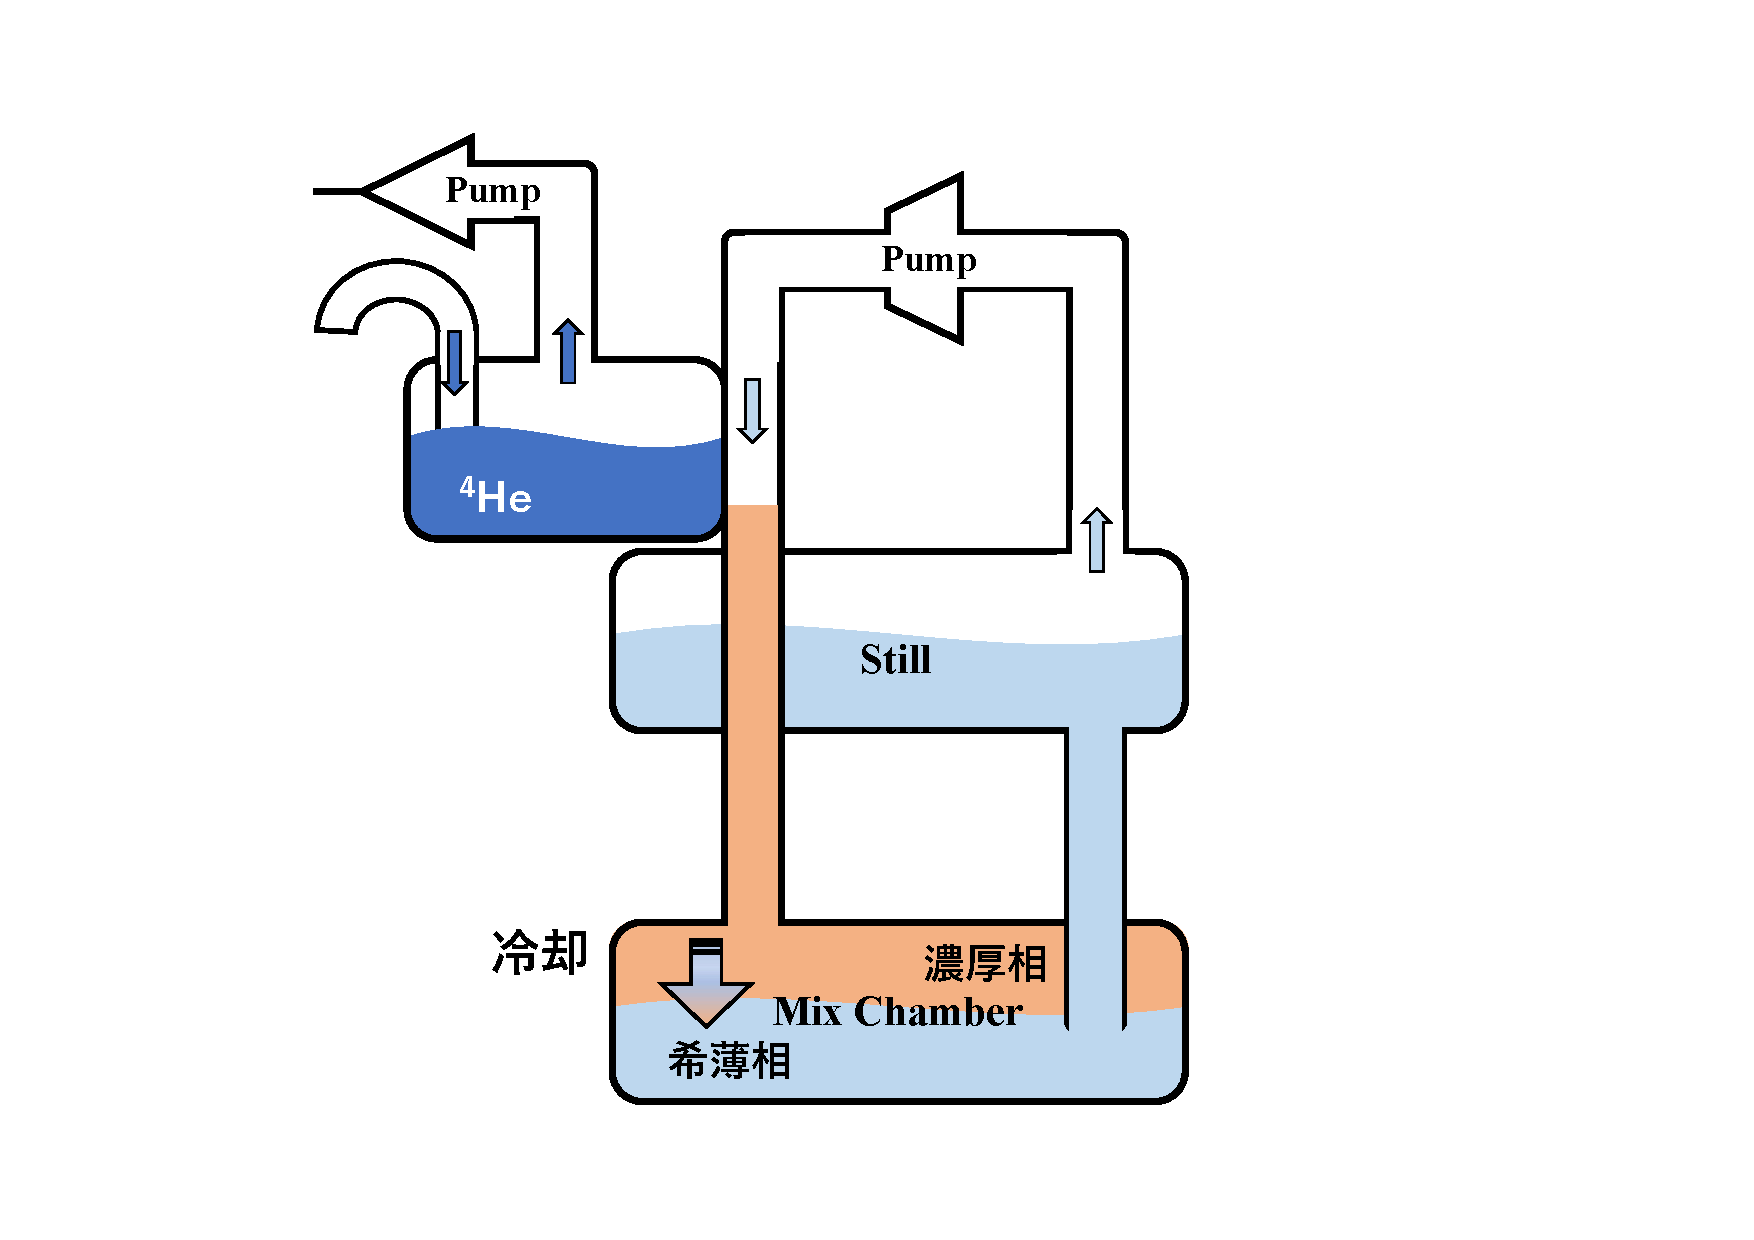
\includegraphics[clip, width=1.0\columnwidth]{fridge.pdf}
            \caption{希釈冷凍機の基本原理}
        \end{minipage}%
        \begin{minipage}[t]{0.4\columnwidth}
            \centering
            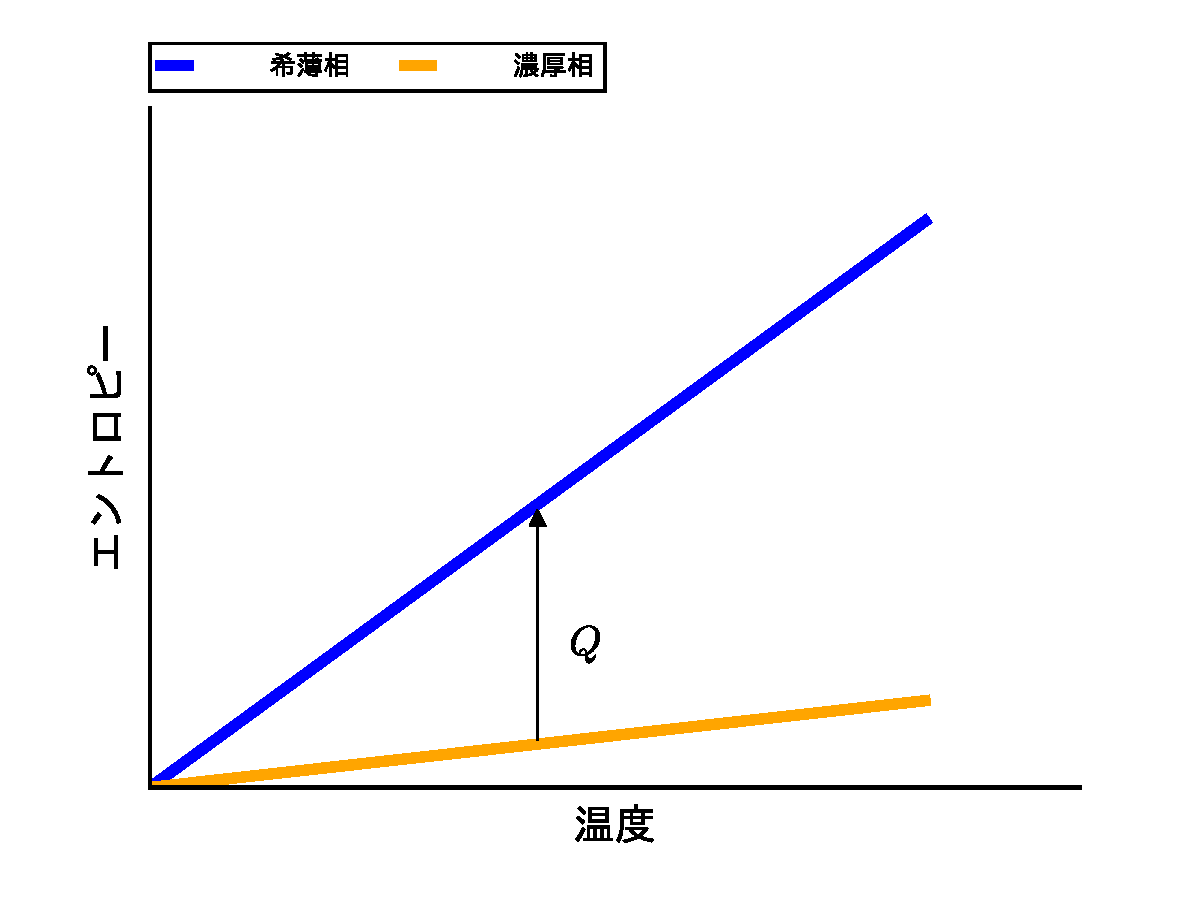
\includegraphics[clip, width=1.0\columnwidth]{entropy.pdf}
            \caption{濃厚相と希薄相のエントロピー}
        \end{minipage}
    \end{figure}
    1K Spot内にはHe4が充填されており排気冷却を行うことで最低温度1Kを実現している。1K Spotの主な役割はHe3を液状にするため冷却機である。次にMix Chamberであるが、この容器内ではHe3とHe4が相分離した状態で混合されている。He3の濃度の小さい相を希薄相、大きな相を濃厚相と呼ぶ。このMix Chamber が希釈冷凍機能を持った心臓部である。希釈冷凍機を構成する最後の1つ、StillではHe3の排気が行われている。冷却の基本原理はHe3を選択的に排気することでHe3を濃厚相から希薄相へと強制的に’蒸発’させることにより生まれる断熱減圧冷却法であるが、STillには希薄相のみが充填されており、He3が選択的に排気されている。右の図では濃厚相と希薄相では希薄相の方がエントロピーの違いを示している。希薄相の方が濃厚相よりもエントロピーが高いため、He3が濃厚相から希薄相へと浸透するとよってHe3外部空から熱を吸収するため,冷却が起こる。排気したHe3は再び濃厚相へと供給され、この繰り返しにより冷凍機内部は10mKまで冷却される。希釈冷凍機の図にあるように、冷凍機内部にはいくつものプレートで区切られており、プレートの熱伝導を利用して、各ステージは段階的に温度が代わっている。最下部のCold Finger内にサンプルを搭載する。サンプルはパーマロイでできた$\mu$metalで蔽うことで外部磁場を遮蔽している。
    \begin{figure}[H]
        \centering
        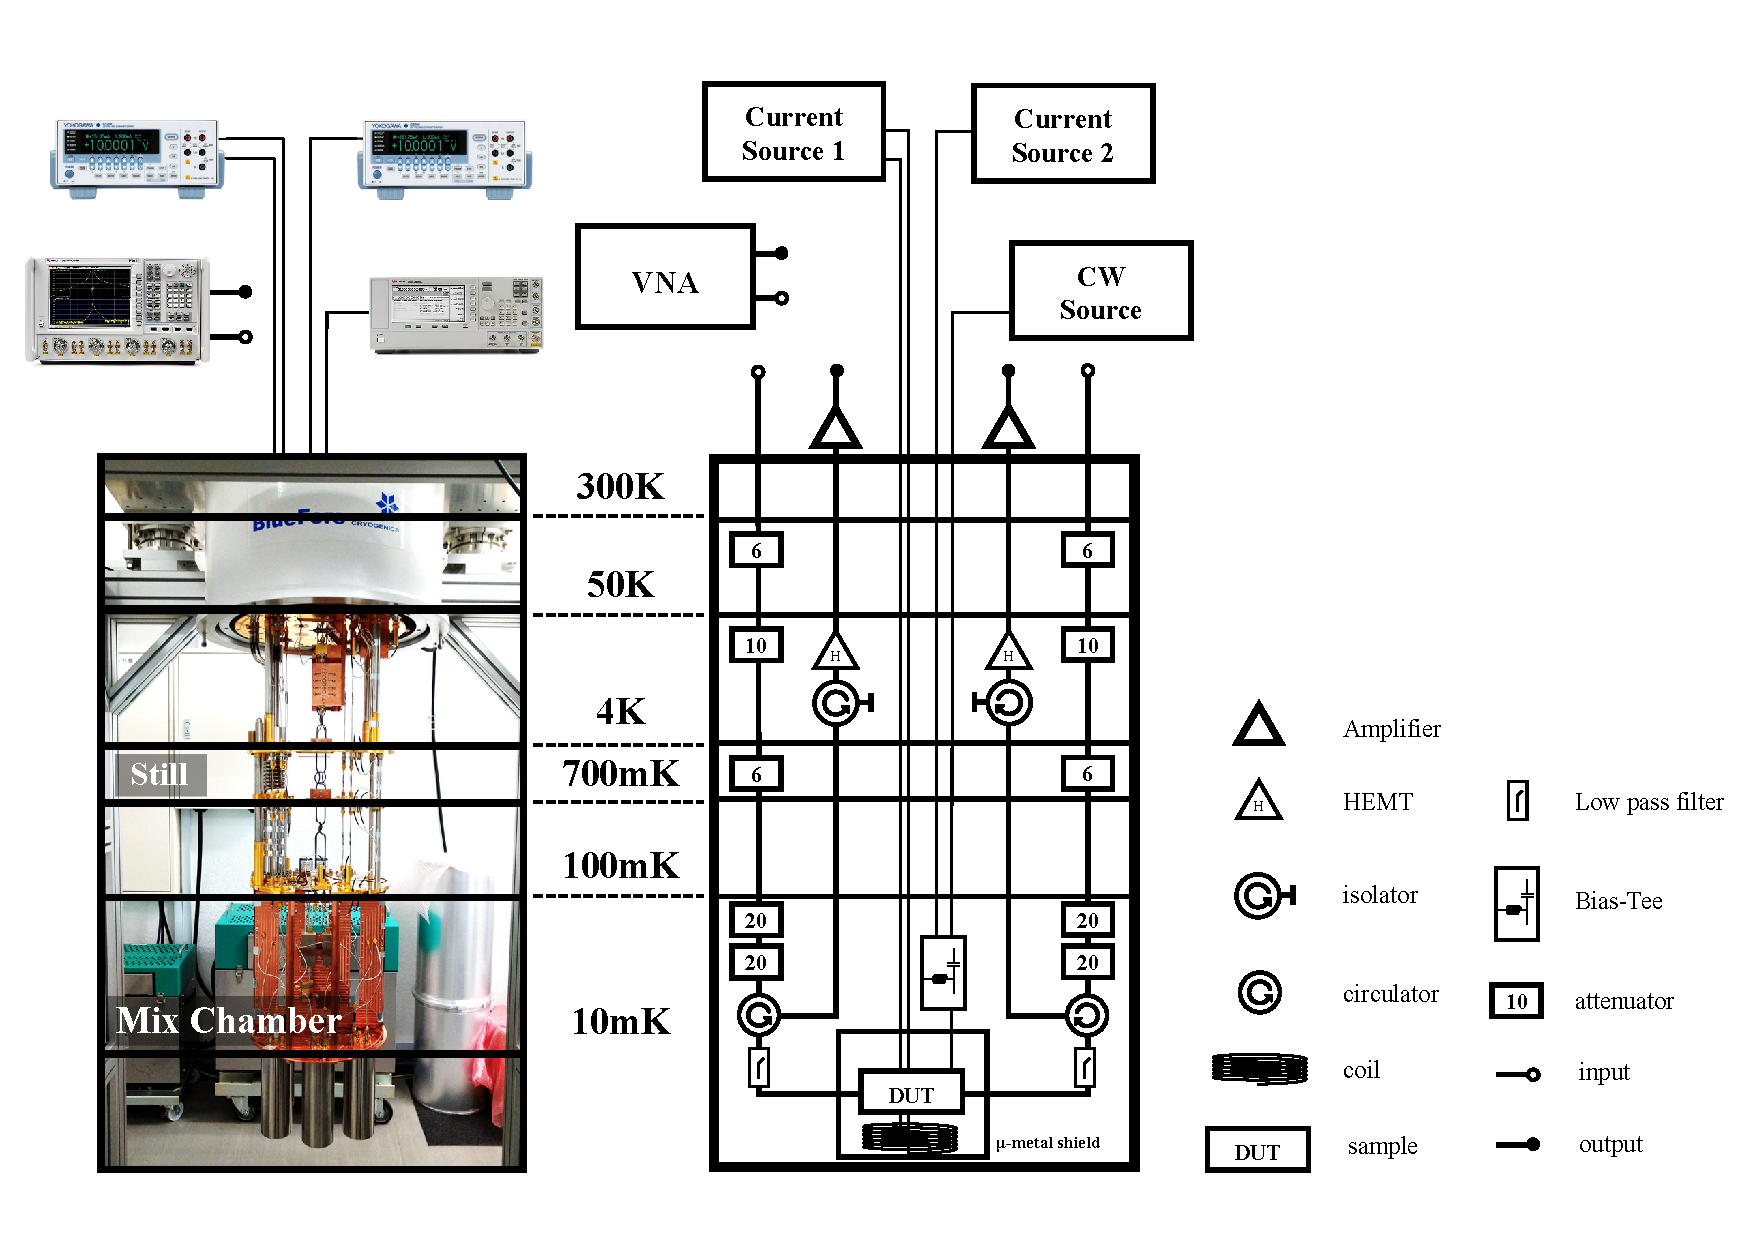
\includegraphics[width=11cm,angle=-90]{fridgesetup2.pdf}
        \caption{希釈冷凍機のセットアップ}
    \end{figure}
    冷凍機内部の部品はアンプやサンプルホルダーに至るまでインピーダンスが50$\Omega$となるように適切に設計、製造されたものを使用している。
    本実験で使用した機材はKeysight社のN5231A PNA-Lマイクロ波ネットワーク・アナライザ、13.5 GHz及びE8257D PSGアナログ信号発生器、100 kHz~67 GHz、横河電気の直流電圧/電流源 GS200である。電流源はサンプルホルダーに搭載されたコイル操作用、サンプルに搭載されたオンチップバイアスラインを操作用の2つを使用した。サンプル自体には2つのポートが存在するが、4~8GHz帯のCirculatorを取り付けることで透過測定及び反射測定が可能となっている。すなわちVNAとサンプルの接続方法は4通り存在し、それぞれについて測定を行った。
    また、冷凍機内には62dBのAttenuator(減衰器)が取り付けられており、ケーブルの減衰7dBも含めるとVNAから出力される信号は総計69dB減衰されることに注意する。

    次にサンプルについて説明する。サンプルとPCBはAlの細線を用いてボンディングされている。サンプルのグランド及びPCBからサンプルへの伝送ラインの接続はこのAl細線により確保されている。

    % \begin{figure}[H]
    %     \centering
    %     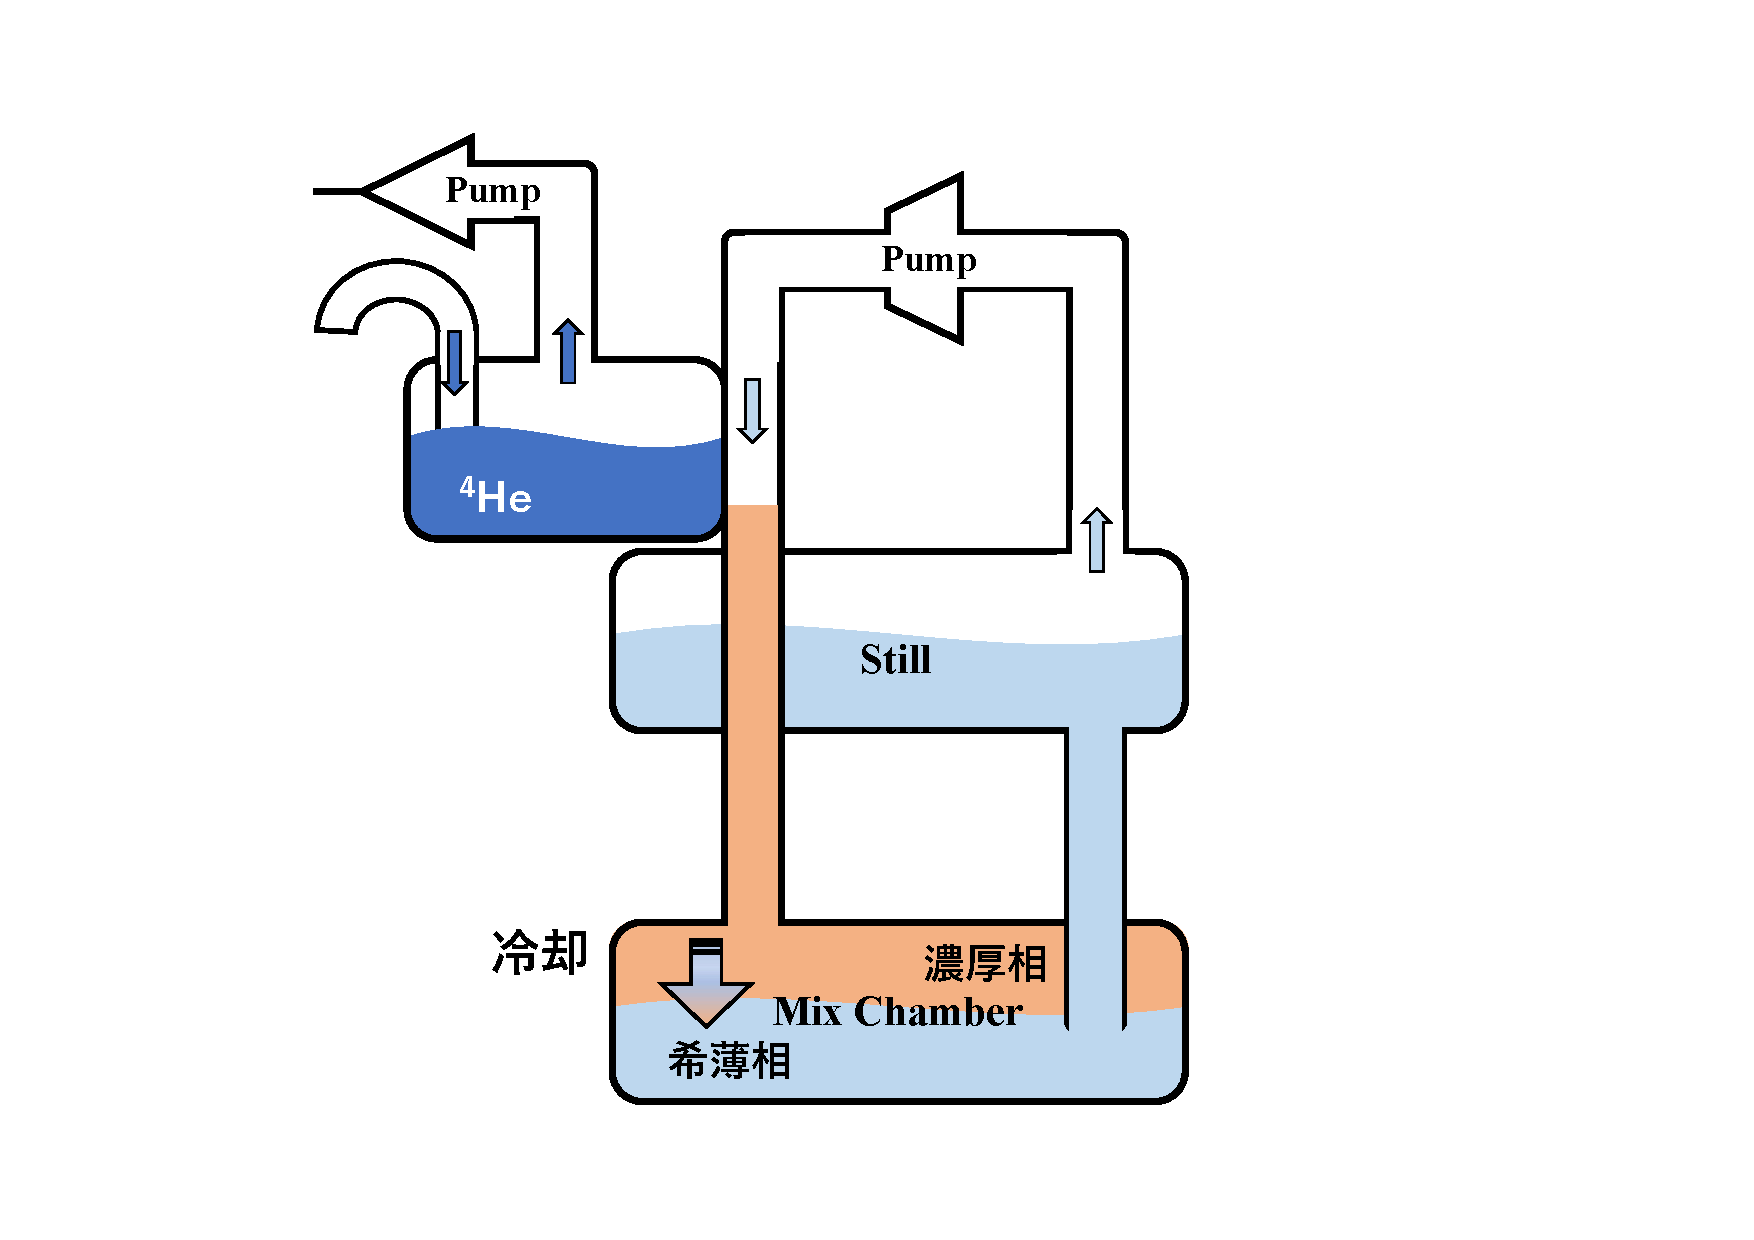
\includegraphics[width=4cm]{fridge.pdf}
    %     \caption{希釈冷凍機のセットアップs}
    % \end{figure}
